\ifx\mybook\undefined
\documentclass[uplatex,dvipdfmx]{jsarticle}
\usepackage{okumacro,plext}
\usepackage{natbib}
\usepackage{url}
\usepackage{txfonts}
\usepackage[utf8]{inputenc}
\usepackage[T1]{fontenc}
%\usepackage{my_resume}
\usepackage{graphicx,wrapfig}
%\usepackage[greek,english]{babel}
%\usepackage{teubner}
%\usepackage[dvipdfm,bookmarkstype=toc=true,pdfauthor={江口聡, EGUCHI Satoshi}, pdftitle={}, pdfsubject={},pdfkeywords={},bookmarks=false, bookmarksopen=false,colorlinks=true,urlcolor=blue,linkcolor=black,citecolor=black,linktocpage=true]{hyperref}
%  \AtBeginDvi{\special{pdf:tounicode EUC-UCS2}}% platex-utf8 でも OK
\author{江口聡}
%\date{}
\title{ベンサム}
\if0 %----------------------------------------------------------------

\fi  %----------------------------------------------------------------
\begin{document}
\maketitle
\else\chapter{功利主義}\fi


\section{ベンサム}

\begin{itemize}
\item Jeremy Bentham (1748--1832)
\item 快楽説。主観的に楽しく生きることがよく生きること。

  \begin{quote}\small{}
    自然は人類を\kenten{苦痛}と\kenten{快楽}という、二人の主権者の支配のもとにおいてきた。われわれが何をしなければならないかということを指示し、またわれわれが何をするであろうかということを決定するのは、ただ苦痛と快楽だけである。一方においては善悪の基準が、他方においては原因と結果の連鎖が、この二つの玉座につながれている。苦痛と幸福とは、われわれのするすべてのこと、われわれの言うすべてのこと、われわれの考えるすべてのことについて、われわれを支配しているのであって、このような従属をはらいのけようとどんなに努力しても、その努力はこのような従属を証明し、確認するのに役だつだけであろう。ある人は、ことばのうえではこのような帝国を放棄したように見せかけるかもしれないが、実際上は依然としてその帝国に従属しつづけている。\citep[邦訳pp. 81-2]{bentham1789:_introd_to_princ_of_moral_and_legis}
  \end{quote}

\end{itemize}


\if0
  \section*{文学と押しピン遊び}

  % \begin{wrapfigure}{r}{50mm}
  %   \begin{center}
  %     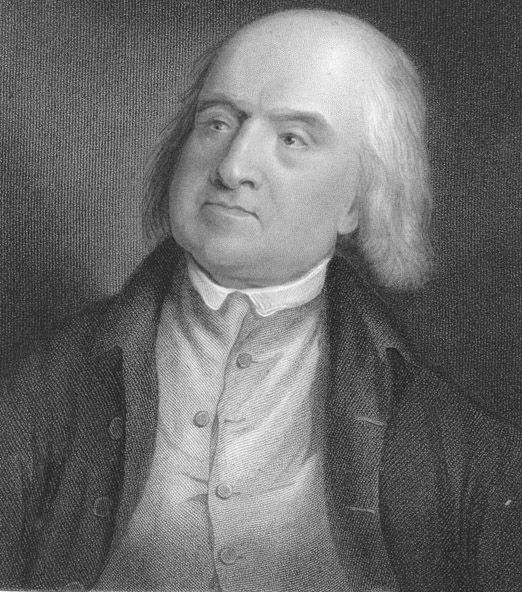
\includegraphics[width=50mm]{images/bentham.jpg}
  %     \caption{Jeremy Bentham}
  %   \end{center}
  % \end{wrapfigure}


\begin{quote}
\small Jeremy Bentham, The Rationale of Reward, Book 3, Chapter 1.からの抄訳。Peter Singer,
  Ethicsにも収録されている。江口聡訳.(c) EGUCHI Satoshi 2006。
\end{quote}

\vspace{2zw} 技芸(arts)と学術(sciences)を、全体として社会の幸福とのかかわりのなかで考察すると、これらは二つの部分に分けることができる。つまり、(1)娯楽(amusement)と好奇心(curiosity)のためのもの、(2)直接的・間接的な有用性のためのものである。人間の知識のこの二つの部門について、政府はまったく別の対処方法を必要とする。

娯楽ための技芸と学問ということで私が言おうとしているのは、ふつうは芸術(fine arts)と呼ばれているものである。たとえば、音楽、文学、絵画、彫刻、建築、造園などである。これらを枚挙することはここでは控えておくことになる。もし、このような枚挙を完全にするためにどうしても必要な形而上学的な議論に深く入りこんでしまえば、現在の論題からあまりにも離れてしまうだろうからである。あらゆる種類の娯楽がこの項目に含まれる。

(中略)

好奇心のための技芸と学術ということで私が言おうとしているのは、実際には快をもたらすが、それは芸術ほどではなく、また、一見したところ我々がそれが快を与えるということを否定したいと思うかもしれないようなものである。これは、これらの好奇心のための技術と知が、教養ある人々にとっては芸術ほどには快をを与えないというわけではない。しかし、これらの技術と知を研究しているひとびとの数の方は限られている。紋章学や純粋年代学(pure chronology){\――}現在は珍奇な言葉の寄せ集めしかもたらさない古代や外国の言語についての知識{\――}といった学問はこうした性質のものである。また古代の風習の研究なども、道徳性に対して応用することのできるなんからの教示や、なにか有益で望ましい知識をもたらさないのならば、この種の性質のものである。

これらすべての技芸と学術{\――}娯楽と好奇心のための技芸と学術の両方について語っているのだが{\――}が持つ価値は、それが生み出す快楽に正確に比例している。ある人々が技芸や学術に認めようと試みているその他の卓越性は、実はまったくのたわごとにすぎない。偏見を離れれば、押しピン遊びは音楽や文学といった技芸や学術と同じ価値がある。もしも押しピン遊びが、より多くの快楽を提供するとすれば、それはより多くの価値があることになろう。文学(poetry)や音楽はほんの少数の人々によってしか楽しまれない。押しピン遊びは常に無害である。同じことが文学についても常に主張できれば好都合だが、実際にはそうではない。実際のところ、文学と真理との間には、本性上の対立がある。それは文学の誤った教訓と虚構性である。文学者は常になにか偽であるものを必要としている。文学者が真理に土台を置くというふりをするときにも、その上にある装飾品はフィクションである。文学者の仕事はわれわれの感情を刺激し、偏見を助長することにある。真実、すなわちあらゆる種類の正確さは、文学者にとっては致命的である。文学者はなにごとも色眼鏡を通して見ねばならず、他の人々にも同じよう色眼鏡を通して見させようとするのである。たしかに、これまで高貴な魂(noble spirits)と呼ぶことのできる人々が存在しており、文学と哲学はともに彼らに多くを負ってきた。しかし、これらの例外は、この文学という魔術が生み出した不幸を償うものではない。もし文学と音楽が押しピン遊びよりも好まれるに値するとすれば、それは、まったく気むずかしい人々を満足させるよう計算されているからに違いない。

\section{快楽計算}
\begin{itemize}
\item 強さ、持続性、確実性、遠近性、多産性、純粋性、範囲が重要。
\item 快楽のリスト。
\end{itemize}

\fi

\section{ベンサムの功利主義}


\begin{itemize}
\item ベンサム、J.S.ミル。
\item 快楽と苦痛が重要。
\item 最大多数の最大幸福。関係者全員の快楽を最大にし、苦痛を最少にする行為・制度が正しい。
\item 各種の制裁をもちいて人々の行動をコントロールする。
\item 19世紀初頭のイギリス「哲学的急進派」の思想的基盤。19世紀後半にかけて、さまざまな社会改革運動に理論的基盤を提供。監獄の改革、婦人参政権を含む普通選挙、自由貿易、植民地制度改革、労働組合の合法化、公費による国民教育、言論出版の自由、秘密投票制、官吏任命制および業績主義、高利禁止法の廃止、地方政府の改革、海運の安全規定、衛生上の改革、公費による予防医療、統計の組織的蒐集、貧困者のための無料裁判、産児制限、煙害対策。
\item ミルの『自由論』。言論の自由と、個性の発展の尊重。
\end{itemize}


\begin{enumerate}
\item J. ベンサム(1748-1832)、J. S. ミル(1806-1873)など。

 \item 功利性の原理。いくつかの行動あるいは社会政策を選択する場合、関係者全員にとって最善の結果をもたらすものを選ばねばならない。「最大多数の最大幸福」。

   \begin{quote}\small{}

     「功利」または「最大幸福の原理」を道徳的行為の基礎として受けいれる信条にしたがえば、行為は、幸福を増す程度に比例して正しく、幸福の逆を生む程度に比例して誤っている。幸福とは快楽を、そして苦痛の不在を意味し、不幸とは苦痛を、そして快楽の喪失を意味する。この説がたてた道徳の標準について明確な意見を述べようとすれば、まだまだ多くのことをいわねばならない。とりわけ、苦痛と快楽の観念の中にどういうものが含まれるのか、どの程度までこれが未解決の問題として残されているかについて触れなければならない。しかし、こういう補足的な説明は、この道徳説がもとづいている人生観{\――}つまり、快楽、および苦痛の不在が、目的として望ましい唯一のものであるという人生観、さらに、ずべての望ましいもの〔それは功利主義においも他説同様たくさんある〕は、その中に含まれた快楽のために、または快楽を増し苦痛を防ぐ手段として、望ましいのだという人生観{\――}には影響を与えない。(ミル『功利主義論』第2章)

   \end{quote}

 \item 単純。平等(「誰もを一人として数え、誰も一人以上に数えない」)

 \item 各種のサンクション(制裁)を用いて、人々をコントロール。

 \item 19世紀初頭のイギリス「哲学的急進派」の思想的基盤。19世紀後半にかけて、さまざまな社会改革運動に理論的基盤を提供。監獄の改革、婦人参政権を含む普通選挙、自由貿易、植民地制度改革、労働組合の合法化、公費による国民教育、言論出版の自由、秘密投票制、官吏任命制および業績主義、高利禁止法の廃止、地方政府の改革、海運の安全規定、衛生上の改革、公費による予防医療、統計の組織的蒐集、貧困者のための無料裁判、産児制限、煙害対策。

\item 現在でも社会政策等に大きな影響。

\end{enumerate}


\section{トクヴィルのデモクラシー論}




\section{J. S. ミルのリベラリズム}

\begin{itemize}
\item 言論表現のほぼ絶対的自由の必要性。
\item (1) 政府批判のため、(2)真理の獲得のため、(3)批判検討のため。
\item 個性の擁護。幸福のためには自由な「生活の実験」による個性の発展が必要。
\end{itemize}

\if0

\begin{quotation} \small{}人類が、不完全であるかぎりは、さまざまな意見のあることが有益であるのと同じく、次のことが有益である。すなわち、さまざまな生活の実験があること、他人への危害がないかぎり自由な活動の場が多種多様な性格に対して与えられること。また、さまざまな生活様式をもし試みるのが適当と思う人があれば実際にやってみてその価値を明らかにすること、が有益である。要するに、第一義的に他人に関係しない事柄においては、個性が自己を主張することが、望ましい。その人自身の性格ではなくてほかの人々の幸福の主要な構成要素の一つであり、かつ個人的社会的進歩のまさに第一の構成要素をなすものが、欠けていることになるのである。・・・

  知覚、判断、識別感情、精神活動、倫理的好悪さえも含めた人間の諸能力は、選択という行為をする際にのみ訓練される。何事であれそうするのが習慣だからといってする人は、なんの選択もしない。彼は最善のものを見わけたり望んだりする練習ができない。肉体的能力と同じように精神的道徳的能力も、使われることによってのみ向上する。ただ、他の人々がするからするというのでは、これらの能力は少しも訓練されない。それはちょうどある事がらを、他の人々がそれを信じているという理由だけで信じるのど同様である。もしある意見の根拠が、その人自身の理性を納得させるものでなえければ、彼の理性はその意見を採用することによって強められはせず、むしろ弱められがちである。そして、行為への誘因が彼自身の感情や性格に一致しないようなものならば、〔愛情や他人の権利が関係していない場合〕それは彼の感情や性格を活発で精力的なものにするかわりに、不活発で鈍いものにするのに大いに役だつのみである。

  自己の生活設計を、自分のかわりに、世間や自分自身が属している世間の一部が選ぶのにまかせる人は、\ruby{猿}{さる}のような模倣能力のほかにはどんな能力も必要としない。自分自身で生活設計を選ぶ人は、彼のすべての能力を使用する。彼は、見る観察力、予測する推理力と判断力、決定に必要な資料を集める活動力、決定する識別力を使わなければならず、いったん決定をくだしたら、自己の熟慮した決定を守る確固とした意思と自制心を使わなければならない。そして、彼はこれらの能力を、自己の行為のうち、みずからの判断と感情にもとづいて決定する部分の大きさに比例して必要とし、また行使するのである。(J. S. ミル『自由論』)
\end{quotation}

\fi






\nocite{bentham1789:_introd_to_princ_of_moral_and_legis}
\nocite{bentham1825:_ration_of_rewar}


\ifx\mybook\undefined
\bibliographystyle{eguchi}  
\bibliography{bib}
\end{document} %----------------------------------------------------------------
\fi






%%% Local Variables:
%%% mode: japanese-latex
%%% TeX-master: t
%%% coding: utf-8
%%% End:
